% =============================================================
%  GNN-SHM for H3 Rocket Fairing — Payload2026
%  Internal progress slides  (2026-06)
% =============================================================
\documentclass[aspectratio=169, 10pt]{beamer}
\usetheme[progressbar=frametitle, block=fill]{metropolis}
\usepackage[T1]{fontenc}
\usepackage{newtxtext, newtxmath}
\usepackage{microtype}
\usepackage{booktabs}
\usepackage{colortbl}
\usepackage{tikz}
\usetikzlibrary{arrows.meta, positioning, shapes.geometric}

% LUH colours
\definecolor{luhblue}{RGB}{0,80,155}
\definecolor{luhgray}{RGB}{128,128,128}
\setbeamercolor{frametitle}{bg=luhblue, fg=white}
\setbeamercolor{progress bar}{fg=luhblue}
\setbeamercolor{alerted text}{fg=luhblue}
\metroset{progressbar=frametitle, block=fill}

\newcommand{\best}[1]{\textbf{\textcolor{luhblue}{#1}}}
\newcommand{\bad}[1]{\textcolor{red}{#1}}

% ---- metadata -----------------------------------------------
\title{GNN-based SHM for H3 Rocket Payload Fairing}
\subtitle{5-class defect detection + PINN regularisation + multitask centroid regression}
\author{Keisuke Nishioka}
\institute{Institut für Kontinuumsmechanik, LUH}
\date{June 2026 — internal progress}
% =============================================================
\begin{document}
\maketitle

% ---- overview -----------------------------------------------
\begin{frame}{Outline}
\tableofcontents
\end{frame}

\section{Problem setup}

\begin{frame}{Structural health monitoring of the H3 Type-S fairing}
\begin{columns}[T]
\begin{column}{0.55\textwidth}
\textbf{Structure:} CFRP / Al-honeycomb sandwich, 1/6 section\\[4pt]
\textbf{FEM mesh:} 10{,}897 nodes, 34 node features\\[4pt]
\textbf{Task:} 5-class node-level defect classification
\begin{itemize}
  \item Class 0 Healthy (99.6\%)
  \item Class 1 Debonding
  \item Class 2 Foreign-object damage (FOD)
  \item Class 3 Impact damage
  \item Class 4 Delamination
\end{itemize}
\vspace{4pt}
\textbf{Dataset:} 700 FEM simulations (560 train / 140 val)\\
\textbf{Metric:} threshold-optimal macro-F1 (OptF1)
\end{column}
\begin{column}{0.43\textwidth}
\centering
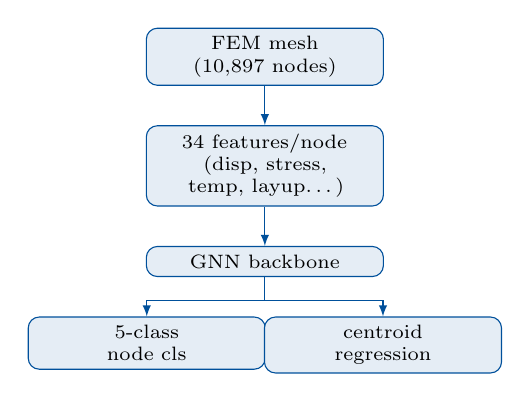
\begin{tikzpicture}[node distance=5mm, every node/.style={font=\scriptsize},
  box/.style={draw=luhblue, fill=luhblue!10, rounded corners, inner sep=3pt, text width=2.8cm, align=center}]
  \node[box] (fem) {FEM mesh (10{,}897 nodes)};
  \node[box, below=of fem] (feat) {34 features/node\\(disp, stress, temp, layup\ldots)};
  \node[box, below=of feat] (gnn) {GNN backbone};
  \node[box, below=of gnn, xshift=-1.5cm] (cls) {5-class\\node cls};
  \node[box, below=of gnn, xshift=1.5cm] (reg) {centroid\\regression};
  \draw[-latex, luhblue] (fem)--(feat);
  \draw[-latex, luhblue] (feat)--(gnn);
  \draw[-latex, luhblue] (gnn.south) -- ++(0,-3mm) -| (cls.north);
  \draw[-latex, luhblue] (gnn.south) -- ++(0,-3mm) -| (reg.north);
\end{tikzpicture}
\end{column}
\end{columns}
\end{frame}

\begin{frame}{Node features (34 dims)}
\small
\begin{tabular}{lll}
\toprule
Dims & Feature group & Physical meaning \\
\midrule
0--2   & Position $(x,y,z)$         & Node coordinates \\
3--5   & Normal $(n_x,n_y,n_z)$     & Surface orientation \\
6--9   & Curvatures $(k_1,k_2,H,K)$ & Shell geometry \\
10--13 & Displacement $(u_x,u_y,u_z,\|u\|)$ & Structural response \\
14     & Temperature                & Thermal loading \\
15--18 & Stress $(s_{11},s_{22},s_{12},\sigma_\text{Mises})$ & Failure indicators \\
19--23 & Principal stress, thermal $\sigma_M$, log-strain & Derived quantities \\
24--30 & Fibre direction, layup (0°/45°/$-$45°/90°) & Anisotropy \\
31--33 & Circumferential angle, boundary/load flags & Topology \\
\bottomrule
\end{tabular}
\end{frame}

\section{Methods}

\begin{frame}{Three modelling additions}
\begin{block}{(A) Multi-task learning — defect centroid regression}
Joint loss: $\mathcal{L} = \mathcal{L}_\text{focal} + \lambda_\text{reg}\,\mathcal{L}_\text{reg}$\\
Shared backbone $\to$ node classification head + graph-level MLP for $(x,y,z)$ centroid.\\
GT centroid computed on-the-fly from defective nodes.
\end{block}
\vspace{4pt}
\begin{block}{(B) Level-1 PINN — stress gradient regularisation}
High predicted defect probability should co-locate with high $|\nabla\sigma_\text{Mises}|$.\\
$\mathcal{L}_\text{stress} = \frac{1}{N}\sum_i p_i^{(\text{def})}\,\exp(-|\Delta\sigma_i|/\sigma_0)$
\end{block}
\vspace{4pt}
\begin{block}{(C) Level-2 PINN — static equilibrium residual $\nabla\!\cdot\!\boldsymbol{\sigma}=0$}
Graph-edge finite differences on $(s_{11},s_{22},s_{12})$; penalises defect predictions
at nodes with low equilibrium violation.
\end{block}
\end{frame}

\begin{frame}{LGSTA — Local-Global Attention GNN}
\textbf{Best-performing architecture:} LocalGlobalAttentionGNN (inspired by LGSTA-GNN, Buildings 2025)
\vspace{0.3em}
\begin{columns}[T]
\begin{column}{0.5\textwidth}
\textbf{Local branch} (GAT $\times$ 4 layers)
\begin{itemize}
  \item Neighbourhood message-passing
  \item Captures local defect boundaries and stress concentrations
\end{itemize}
\vspace{6pt}
\textbf{Global branch} (Multi-head self-attention)
\begin{itemize}
  \item Full $N \times N$ attention over all 10{,}897 nodes
  \item Captures global mode shapes and structural coupling
\end{itemize}
\vspace{6pt}
\textbf{Fusion:} gated combination of both representations
\end{column}
\begin{column}{0.48\textwidth}
\centering
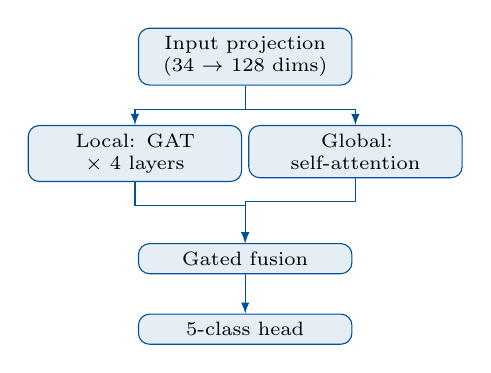
\begin{tikzpicture}[node distance=5mm, font=\scriptsize,
  box/.style={draw=luhblue, fill=luhblue!10, rounded corners, inner sep=3pt, text width=2.5cm, align=center}]
  \node[box] (in) {Input projection\\(34 $\to$ 128 dims)};
  \node[box, below=of in, xshift=-1.4cm] (loc) {Local: GAT\\$\times$ 4 layers};
  \node[box, below=of in, xshift=1.4cm] (glb) {Global:\\self-attention};
  \node[box, below=2.0cm of in] (fus) {Gated fusion};
  \node[box, below=of fus] (out) {5-class head};
  \draw[-latex, luhblue] (in.south) -- ++(0,-3mm) -| (loc.north);
  \draw[-latex, luhblue] (in.south) -- ++(0,-3mm) -| (glb.north);
  \draw[-latex, luhblue] (loc.south) -- ++(0,-3mm) -| (fus.north);
  \draw[-latex, luhblue] (glb.south) -- ++(0,-3mm) -| (fus.north);
  \draw[-latex, luhblue] (fus)--(out);
\end{tikzpicture}
\end{column}
\end{columns}
\vspace{4pt}
{\footnotesize\textcolor{luhgray}{Memory: $O(N^2)$ global attention requires batch size = 1 on 24\,GB GPU.}}
\end{frame}

\section{Results}

\begin{frame}{Architecture \& method comparison (interim, ep\,40--100)}
\centering
\small
\begin{tabular}{llccccccc}
\toprule
Model & Task & OptF1 & AUC & deb & fod & imp & del & Reg.\,RMSE \\
\midrule
\best{LGSTA} & NC+L1+L2 & \best{0.862} & 0.999 & 0.426 & 0.414 & 0.357 & 0.277 & --- \\
SAGE     & NC+L2    & 0.845 & 0.999 & 0.298 & 0.381 & 0.404 & 0.002 & --- \\
\best{LGSTA} & MT+L1+L2 & 0.837 & 0.999 & 0.361 & 0.388 & 0.363 & 0.241 & \best{0.8\,mm} \\
GATv2    & MT+L1+L2 & 0.829 & 0.999 & 0.342 & 0.315 & 0.359 & 0.000 & 0.7\,mm \\
SAGE     & MT+L1+L2 & 0.826 & 0.999 & 0.324 & 0.394 & 0.348 & 0.182 & 0.7\,mm \\
GCN      & MT+L1+L2 & 0.819 & 0.999 & 0.486 & 0.502 & 0.082 & 0.584 & 0.6\,mm \\
GIN      & MT+L1+L2 & 0.812 & 0.998 & 0.186 & 0.000 & 0.260 & 0.030 & 1.2\,mm \\
\bad{Transolver} & MT+L1+L2 & \bad{0.010} & \bad{0.493} & --- & --- & --- & --- & --- \\
\bottomrule
\end{tabular}
\vspace{0.4em}
\begin{itemize}
  \item \textbf{NC} = node classification only \quad \textbf{MT} = multitask (+centroid regression)
  \item \textbf{L1} = stress-gradient PINN \quad \textbf{L2} = equilibrium-residual PINN
  \item Results at ep\,40--100; training continues to 200 epochs
\end{itemize}
\end{frame}

\begin{frame}{Key findings}
\begin{block}{1. LGSTA wins at 0.862 OptF1}
Dual local-global attention captures both \emph{local} stress concentrations and \emph{global} structural coupling — especially important for detecting delamination patterns.
\end{block}
\vspace{4pt}
\begin{block}{2. Multitask centroid regression converges to $\sim$0.7--1.2\,mm RMSE}
With a single shared backbone, the model simultaneously classifies defect nodes \emph{and} locates the defect centroid to sub-mm accuracy (normalised by 5{,}000\,mm structure). Direct use in maintenance planning.
\end{block}
\vspace{4pt}
\begin{block}{3. L2 PINN alone (SAGE, 0.845) is competitive with L1+L2}
Static equilibrium residual $\nabla\!\cdot\!\boldsymbol{\sigma}=0$ provides effective physics regularisation even without the stress-gradient term.
\end{block}
\vspace{4pt}
\begin{alertblock}{Negative: Transolver collapses (AUC $\approx$ 0.49)}
Transolver is designed for structured grids; it fails on the irregular FEM mesh topology even without physics losses.
\end{alertblock}
\end{frame}

\section{Outlook}

\begin{frame}{Next steps}
\begin{itemize}
  \item \textbf{Finish 200-epoch runs} — GCN, GIN, LGSTA, GATv2, MeshGNN convergence
  \item \textbf{Level-3 PINN} — wave phase consistency $\angle(\hat{u}_j\hat{u}_i^*)=\omega|dx|/c$ once guided-wave dataset expanded beyond 6 defect samples
  \item \textbf{Cross-structure evaluation} — train on fairing Section~1, test on Section~2 (OOD geometry)
  \item \textbf{Experimental data} — transfer to TSA / DIC measurements for sim-to-real gap analysis
\end{itemize}
\vspace{0.5em}
\begin{block}{Target for WCCM meeting (2026-06-23)}
Final results table with all 8 architectures at 200 epochs + ablation:
NC vs.\ MT, L1 vs.\ L2 vs.\ L1+L2.
\end{block}
\end{frame}

\end{document}
